
% 2D Vector Rotation
%
% File:         2d-vector-rotation.tex
% Author:       Bob Walton (walton@acm.org)
% Date:      	Fri Dec 21 03:00:58 EST 2012
  
\documentclass{minimal}
\usepackage[paperheight=2.4in,paperwidth=2.4in,
            height=2.4in,hoffset=0.0in,
	    voffset=0.05in,left=0in,width=2.4in]{geometry}
\usepackage{color}
\usepackage[usenames]{xcolor}
\usepackage{scalefnt}
\usepackage[greek,english]{babel}
\usepackage{tikz}
\newcommand{\SMALL}{\scalefont{0.8}}
\newcommand{\THETA}{{\greektext J}}
\usetikzlibrary{arrows}
\begin{document}
\raggedright
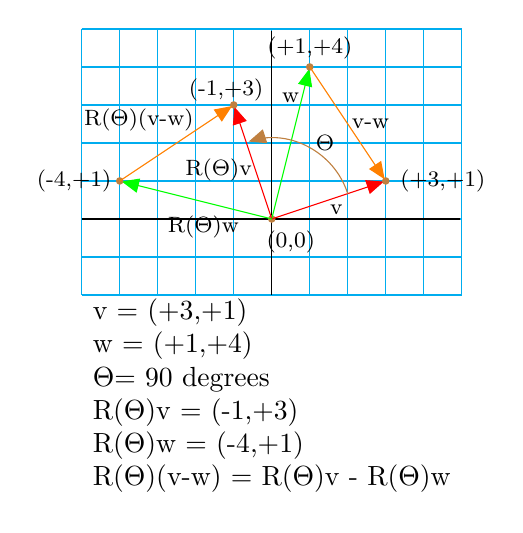
\begin{tikzpicture}[x=0.190in,y=0.190in]
\begin{scope}[yshift=1in,>=triangle 45,shorten >=0.01in]
    \draw[cyan] (-5,-2) grid[step=1] (5,5);
    \draw[black] (-5,0) -- (+5,0);
    \draw[black] (0,-2) -- (0,+5);

    \fill[brown] (0,0) circle(0.1) + (+0.5,-0.6) node[black]{\SMALL (0,0)};

    \draw[red,->] (0,0) -- (+3,+1);
    \draw[black] (1.7,0.25) node{\SMALL v};
    \fill[brown] (+3,+1) circle(0.1) + (+1.5,0) node[black]{\SMALL (+3,+1)};

    \draw[green,->] (0,0) -- (+1,+4);
    \draw[black] (+0.5,3.2) node{\SMALL w};
    \fill[brown] (+1,+4) circle(0.1) + (+0.0,+0.5) node[black]{\SMALL (+1,+4)};

    \draw[orange,->] (+1,+4) -- (+3,+1);
    \draw[black] (+2.6,2.5) node{\SMALL v-w};

    \draw[red,->] (0,0) -- (-1,+3);
    \draw[black] (-1.4,1.3) node{\SMALL R(\THETA)v};
    \fill[brown] (-1,+3) circle(0.1) + (-0.2,+0.4) node[black]{\SMALL (-1,+3)};

    \draw[green,->] (0,0) -- (-4,+1);
    \draw[black] (-1.8,-0.2) node{\SMALL R(\THETA)w};
    \fill[brown] (-4,+1) circle(0.1) + (-1.2,0) node[black]{\SMALL (-4,+1)};

    \draw[orange,->] (-4,+1) -- (-1,+3);
    \draw[black] (-3.5,+2.6) node{\SMALL R(\THETA)(v-w)};

    \draw[brown,->] (2,0.6666667) arc(18:108:2.108185);
    \draw[black] (+1.4,2.0) node{\SMALL \THETA};
\end{scope}

\begin{scope}
\draw (0,0.6) node {
    \begin{tabular}[t]{l}
    v = (+3,+1) \\
    w = (+1,+4) \\
    \THETA = 90 degrees \\
    R(\THETA)v = (-1,+3) \\
    R(\THETA)w = (-4,+1) \\
    R(\THETA)(v-w) = R(\THETA)v - R(\THETA)w \\
    \end{tabular}
    };
\end{scope}
\end{tikzpicture}
\end{document}


